\section{Performance Ratio}

Power and energy calculations take into account solar cell performance ratio $PR$, also known as the coefficient for losses. $PR$ components are taken from Mars PV literature:

\begin{enumerate}[(a)]
  \item\label{itm:pr:perm_loss}After deployment, \SI{5}{\percent} permanent dust power loss \citepower{McNatt2016}.
  \item\label{itm:pr:temp}Solar cell efficiency varies by \SI{3}{\percent} due to changing temperature and red-shift spectral losses through the day time-period \citepower{Kerslake1999}.
  \item\label{itm:pr:deposition}Dust deposition degrade the performance at a rate of \SI{0.28}{\percent} per sol during the initial 30 Sols of a mission and long-term degradation is about \SI{0.14}{\percent} per sol \citepower{Landis2004}.
  \item\label{itm:pr:saturation}Dust performance degradiation saturates at about \SI{30}{\percent} \citepower{Stella2005}.
  \item\label{itm:pr:shadowing}Variable shadowing from protruding rover structures \citepower{Stella2005} and terrain masking \citepower{Kerslake1999}.
\end{enumerate}

The components used for $PR$ in the daily energy calculations throughout this chapter will initially be made up of degradation coefficients from (\ref{itm:pr:perm_loss}) and
(\ref{itm:pr:temp}) where validation against MER Opportunity data will use the solar array dust factor reported by the rover rather than those described in (\ref{itm:pr:deposition}) and (\ref{itm:pr:saturation}). Losses from (\ref{itm:pr:shadowing}) and other unaccounted factors will be initially assumed at \SI{5}{\percent} and then iteratively revised along with the solar array dust factor so that the error margin range may be reduced.

Dust deposition induced losses do not perennially degrade the solar cells but fluctuate due to probabilistic dust cleaning events such as encounters with dust devils, storm winds, or even from a steep tilt angle as seen in Figure \ref{fig:image:mer-opportunity-dust-streaks}.

\begin{figure}[h]
  \centering
  \hypersetup{linkcolor=captionTextColor}
  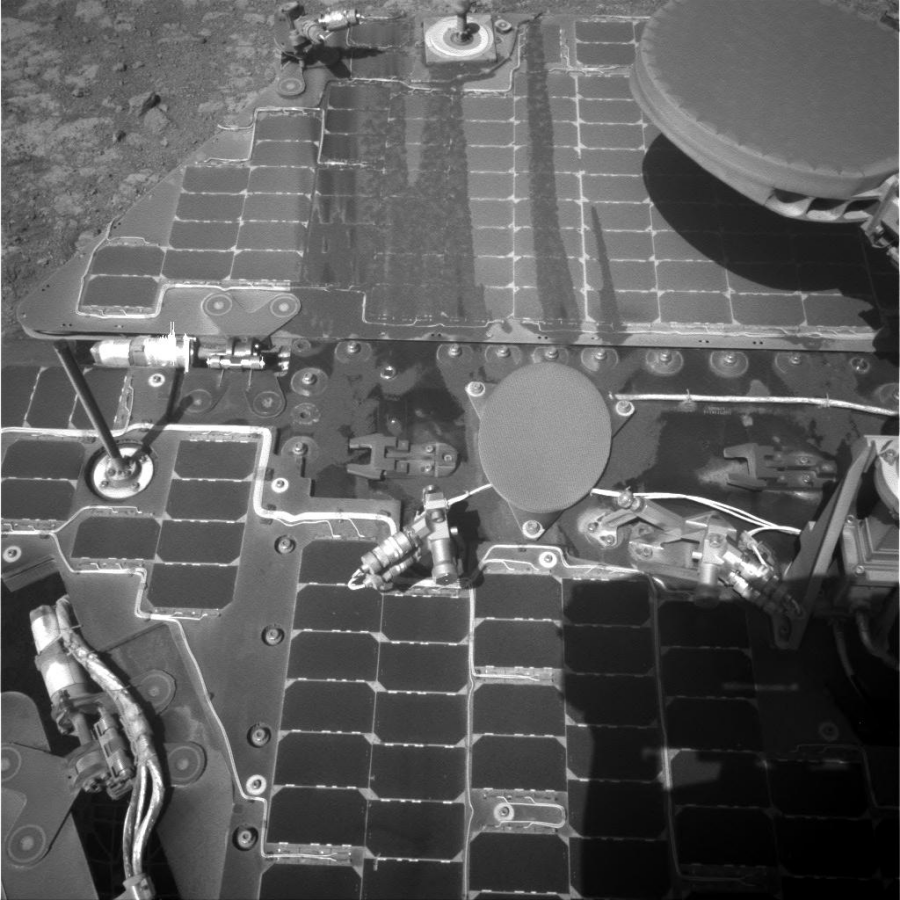
\includegraphics[width=0.6\linewidth]{sections/power-and-energy-predictions/images/mer-opportunity-dust-streaks.png}\\
  \caption[Streak of dust on MER Opportunity's rear solar array during a steep tilt]
          {During a forward, uphill drive on Sol 4311 (March 10, 2016), Opportunity's tilt reached \SI{32}{\degree}. Vibrations from wheels slipping against the ground caused dust to streak down from MER Opportunity's rear solar array while the rover was steeply tilted. Image taken on Sol 4322 (March 21, 2016). Credits: NASA/JPL-Caltech.}
  \label{fig:image:mer-opportunity-dust-streaks}
\end{figure}
% Source: https://www.nasa.gov/feature/jpl/rover-takes-on-steepest-slope-ever-tried-on-mars

\clearpage
\section{Predictions}
\label{sec:PowerAndEnergyPredictions:Predictions}

The power output $P$ generated from a photovoltaic system is measured in watts (\si{\watt}) and is obtained from the global irradiance $G_{h}$ captured by its solar cells:

\begin{equation}
  \label{eq:SA_power}
  P = A \cdot \eta \cdot G_{h} \cdot PR
\end{equation}

where $A$ is the solar cell coverage area $\eta$ their efficiency.

The generated daily energy output $E$ is measured in watt-hours (\si{\watt\hour}) and is obtained from the daily global insolation $H_{h}$ captured by solar cells:

\begin{equation}
  \label{eq:SA_energy}
  E = A \cdot \eta \cdot H_{h} \cdot PR
\end{equation}

Power and energy calculations for inclined solar arrays are obtained from $G_{\beta}$ and $I_{\beta}$ and are denoted as $P_{\beta}$ and $E_{\beta}$ respectively:

\begin{equation}
  \label{eq:SA_slope_power}
  P_{\beta} = A \cdot \eta \cdot G_{\beta} \cdot PR
\end{equation}


\begin{equation}
  \label{eq:SA_slope_energy}
  E_{\beta} = A \cdot \eta \cdot H_{\beta} \cdot PR
\end{equation}

It is worth emphasizing the difference between PV cell, panel/module, and array surface areas in order to emphasize the correct parameter when calculating generated power and energy. PV cells are interconnected together in a package called a panel, or module, which is then wired in series and parallel into a PV array. The interconnections between cells and wiring between panels introduce cell coverage gaps from which no power is generated. As such, considering panel or array rather than cell surface area for power and energy calculations would result in over-estimated values. By way of example, we consider the solar arrays on MER rovers in Figure \ref{fig:image:mer-solar-arrays} which is made up of a total of 499 cells: 165 on the port wing, 167 on the starboard wing, 102 on the stern, and 65 on the body. A cell's dimension is $\SI{3.95}{\centi\meter} \times \SI{6.89}{\centi\meter}$ with two cropped corners. This provides an active area of \SI{26.6}{\centi\meter\squared} thus the solar cell coverage area is $499 \times \SI{26.6}{\centi\meter\squared} = \SI{1.3}{\meter\squared}$.

\todo[inline]{TODO: Source E-mail exchange with Richard C. Ewell (NASA/JPL) for the MER solar cell size.}

\begin{figure}[h]
  \centering
  \hypersetup{linkcolor=captionTextColor}
  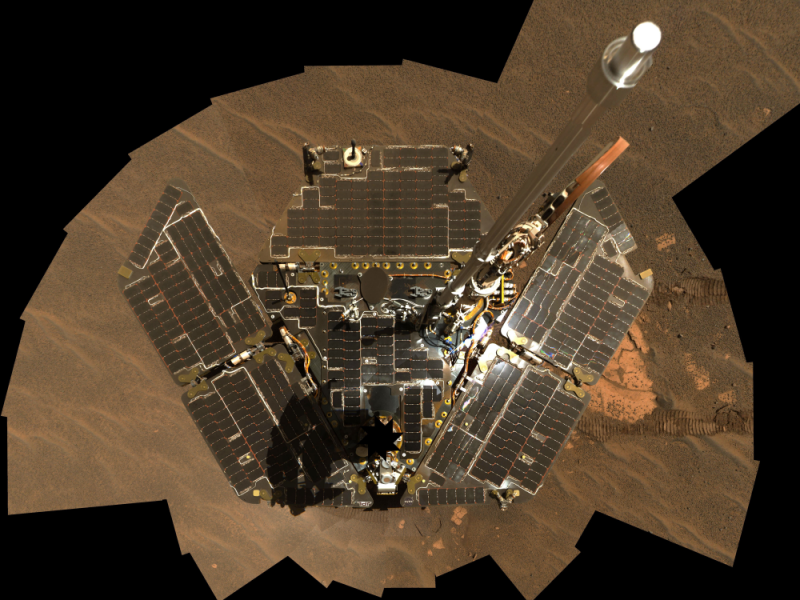
\includegraphics[width=0.8\linewidth]{sections/power-and-energy-predictions/images/mer-solar-arrays.png}\\
  \caption[MER solar arrays]
          {MER solar arrays. Credits: NASA/JPL-Caltech/Cornell.}
  \label{fig:image:mer-solar-arrays}
\end{figure}
% Source: https://mars.nasa.gov/resources/5852/opportunity-self-portrait/?site=insight

\clearpage
\section{Validation}
\label{sec:PowerAndEnergyPredictions:Validation}

\todo[inline]{TODO: Short intro text? Why are we validating? Explain that the equations we are using were based on Viking Lander data and we need to verify if it is still robust today by validating it against the wealth of data we've accumulated since, specifically with MER Opportunity data which is illustrative of mobile rover missions rather than a stationary lander mission.}

\subsection{Horizontal Surface}
\label{sec:PowerAndEnergyPredictions:Validation:HorizontalSurface}

In order to validate the formulas presented in Section \ref{sec:PowerAndEnergyPredictions:Predictions}, MER Opportunity status update parameters were applied to the daily energy calculation presented in Equation \ref{eq:SA_energy}. The following data was scraped from the rover's status update website for Mars years MY29 through MY33:

\begin{enumerate}[(a)]
  \item Sol: the mission's Martian day when the status report was made.
  \item Terrestrial date: the date on Earth when the status report was made.
  \item Atmospheric opacity: the $\tau$ factor introduced in Section \ref{sec:MartianEnvironment:Dust:AtmosphericOpacity}.
  \item Solar Array dust factor: a value between 0 and 1 with the latter represents perfectly clean solar arrays.
  \item Daily energy production: in watt-hours (\si{\watt\hour}).
\end{enumerate}

For the purpose of insolation calculations, the areocentric longitude $L_{s}$ was determined from the terrestrial date based on the process and equations in \citeother{Allison2000}. The resulting predicted energy production was then compared to the rover's reported daily energy production. These are presented for selected Mars years in Figure \ref{fig:plot:mer-energy-production-predicted-vs-reported}.

\begin{figure}[h]
\captionsetup[subfigure]{justification=centering}
\vspace{-2ex}
	\centering
    %% setup sizes
    \setlength{\subfigureWidth}{0.50\textwidth}
    \setlength{\graphicsHeight}{80mm}
    %% kill hyper-link highlighting
    \hypersetup{hidelinks=true}%
    %% the figures
%% 1st row
  	\begin{subfigure}[t]{\subfigureWidth}
      \centering
  		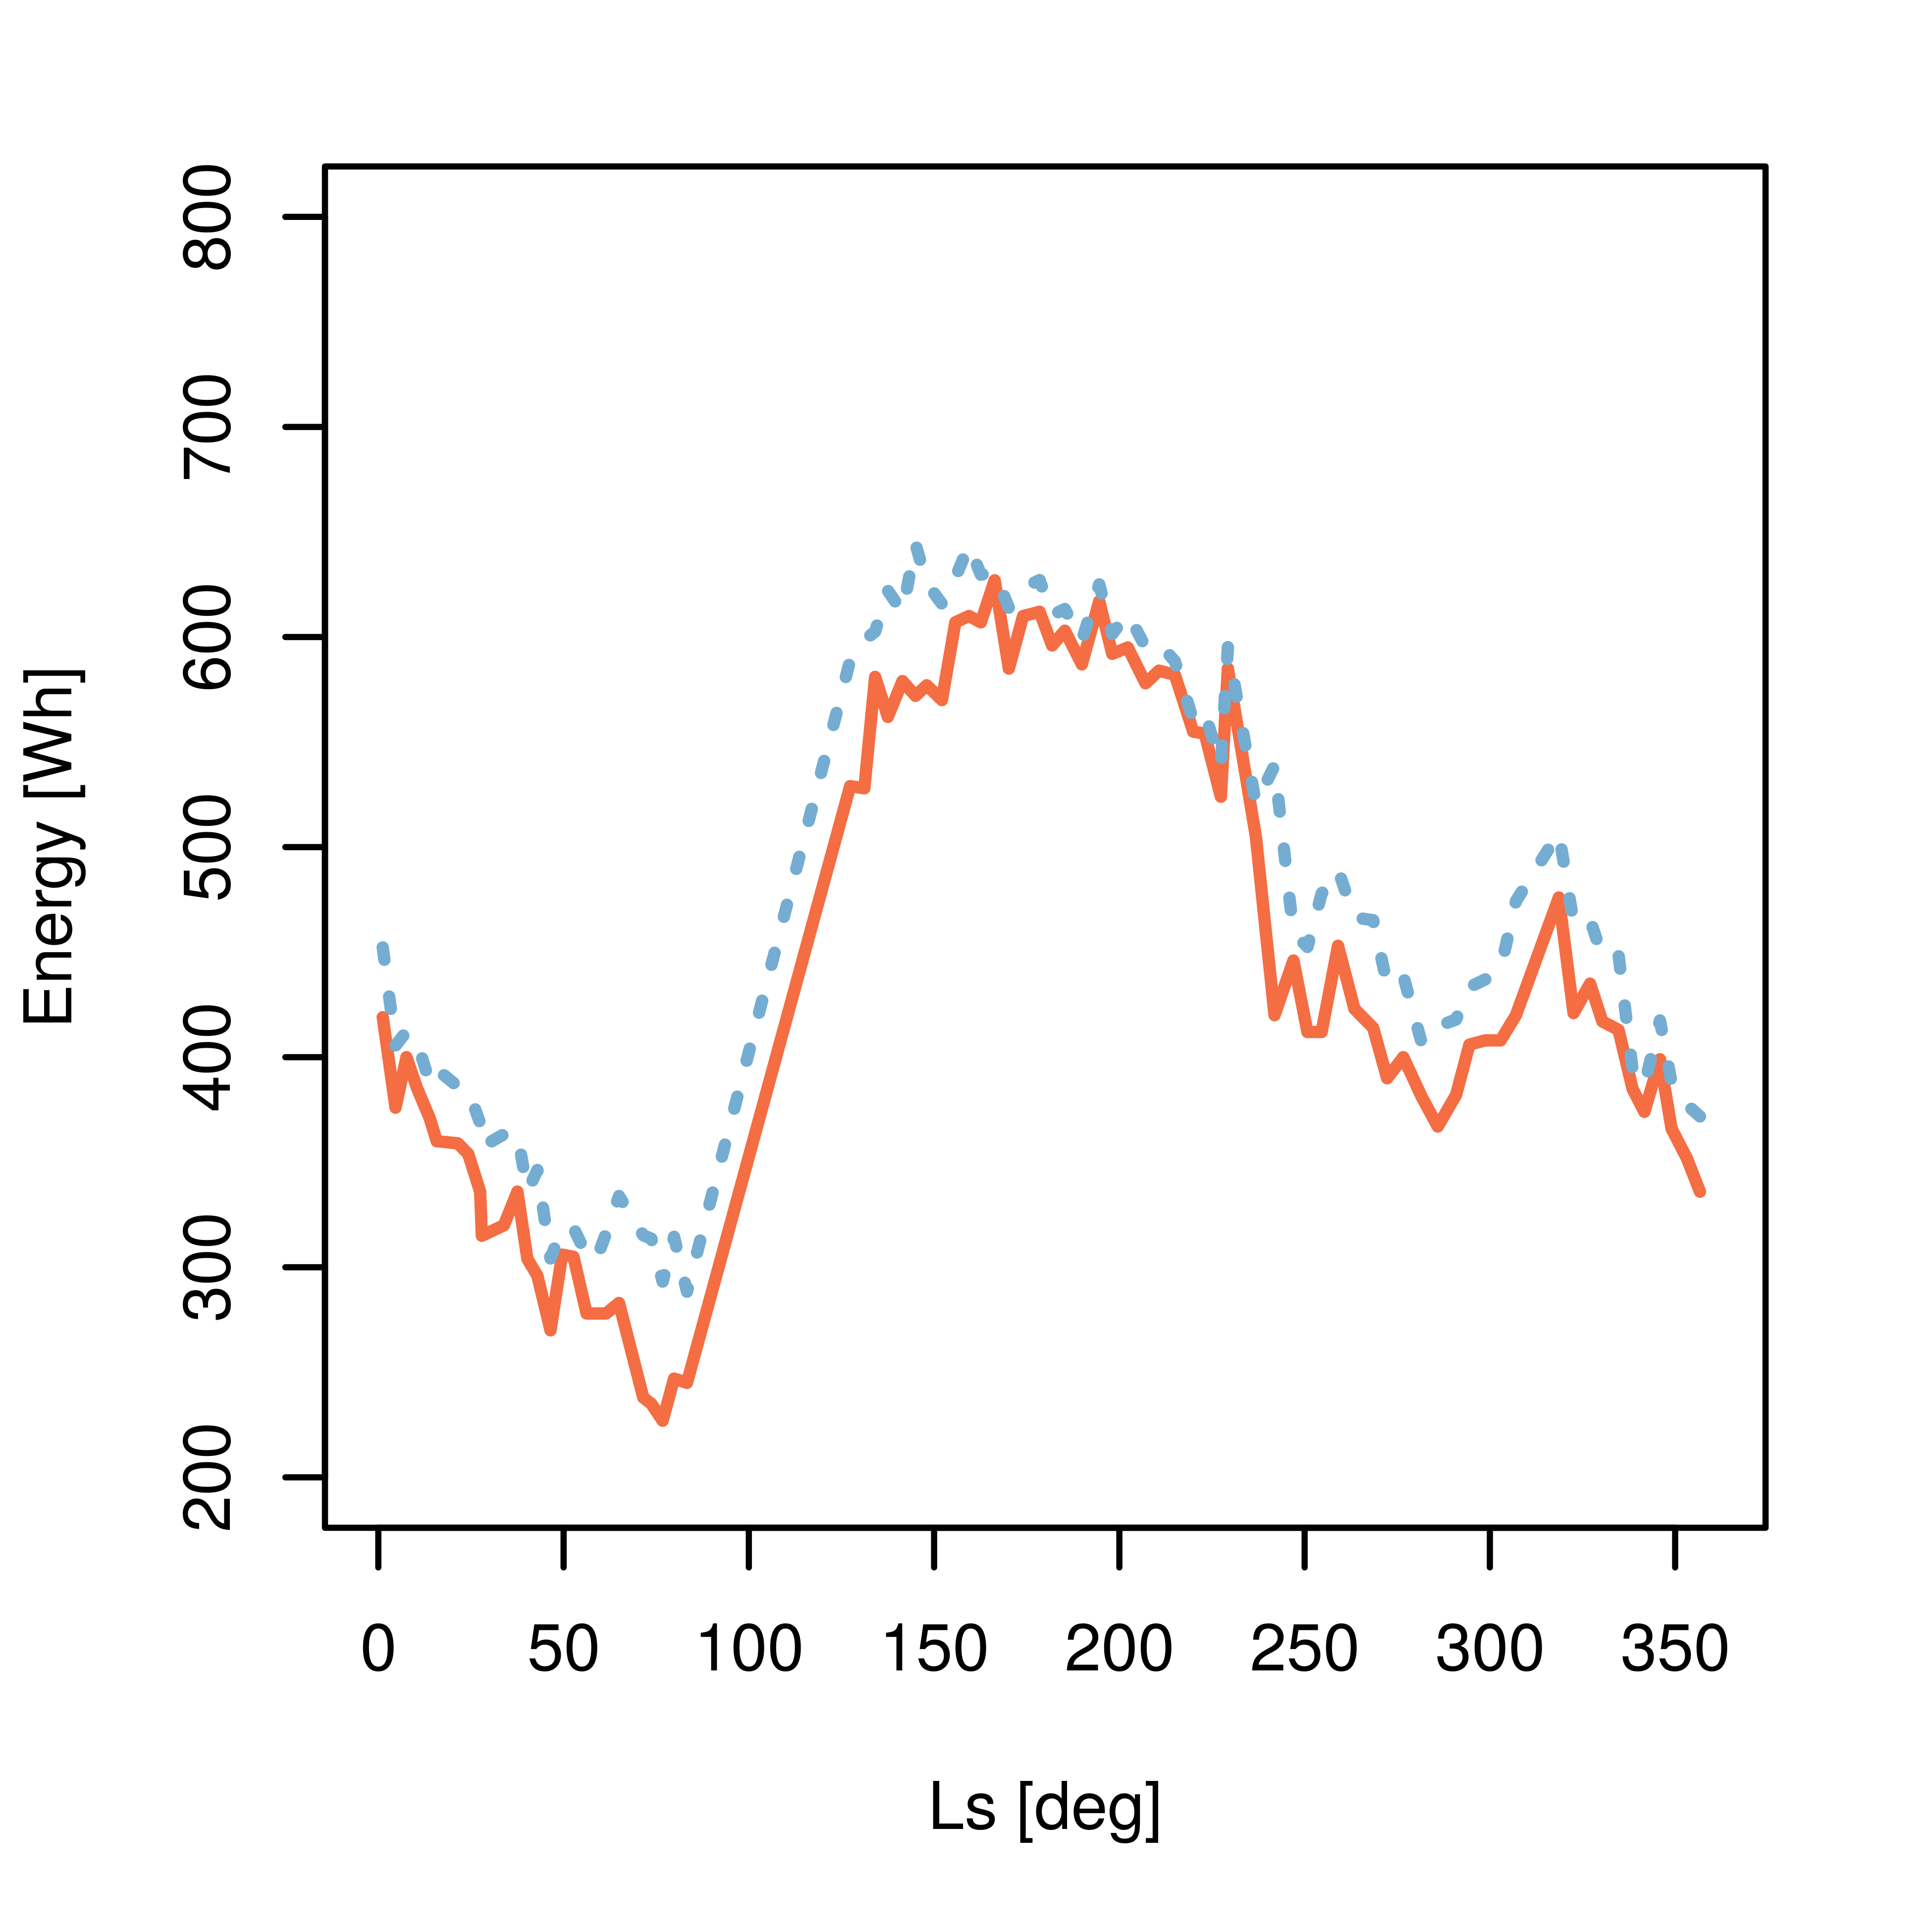
\includegraphics[height=\graphicsHeight]{sections/power-and-energy-predictions/plots/predicted-vs-measured-energy-my29.png}
  		\subcaption{MY29}
  		\label{fig:plot:sub:mer-energy-production-predicted-vs-reported-my29}
  	\end{subfigure}\hfill
    \begin{subfigure}[t]{\subfigureWidth}
      \centering
  		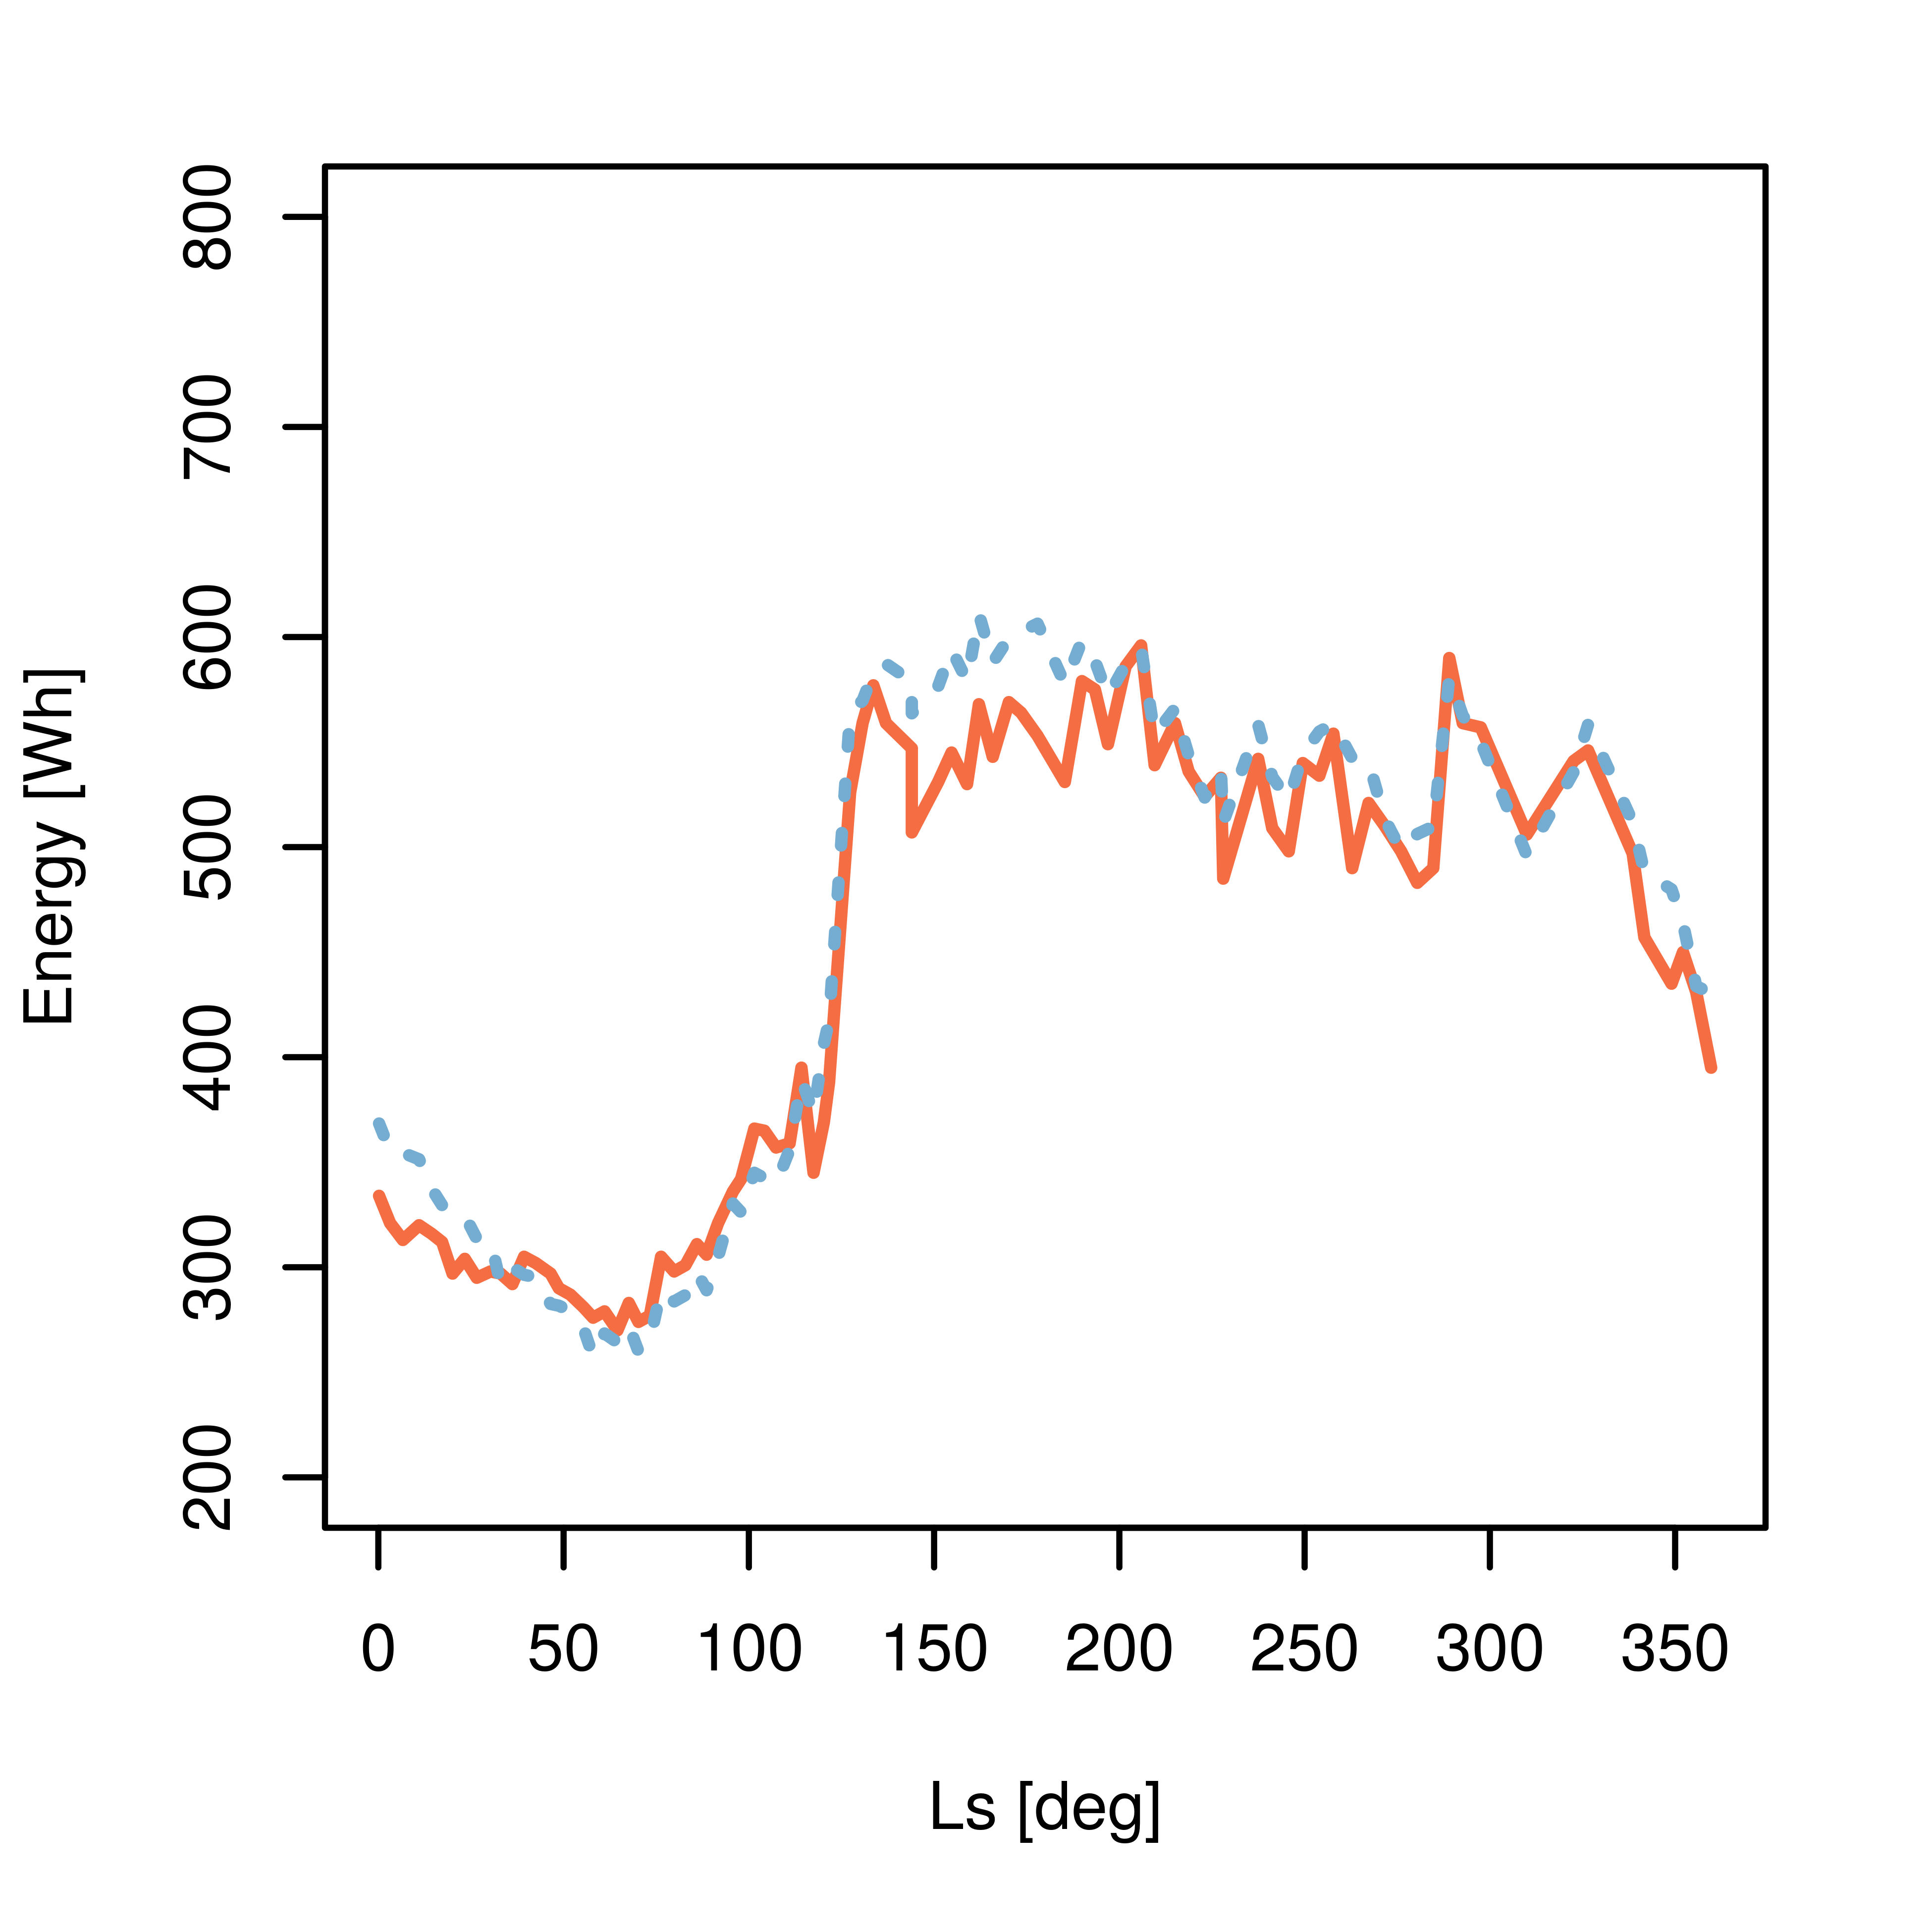
\includegraphics[height=\graphicsHeight]{sections/power-and-energy-predictions/plots/predicted-vs-measured-energy-my30.png}
  		\subcaption{MY30}
  		\label{fig:plot:sub:mer-energy-production-predicted-vs-reported-my30}
  	\end{subfigure}\\[0.8ex]
%% 2nd row
    \begin{subfigure}[t]{\subfigureWidth}
      \centering
  		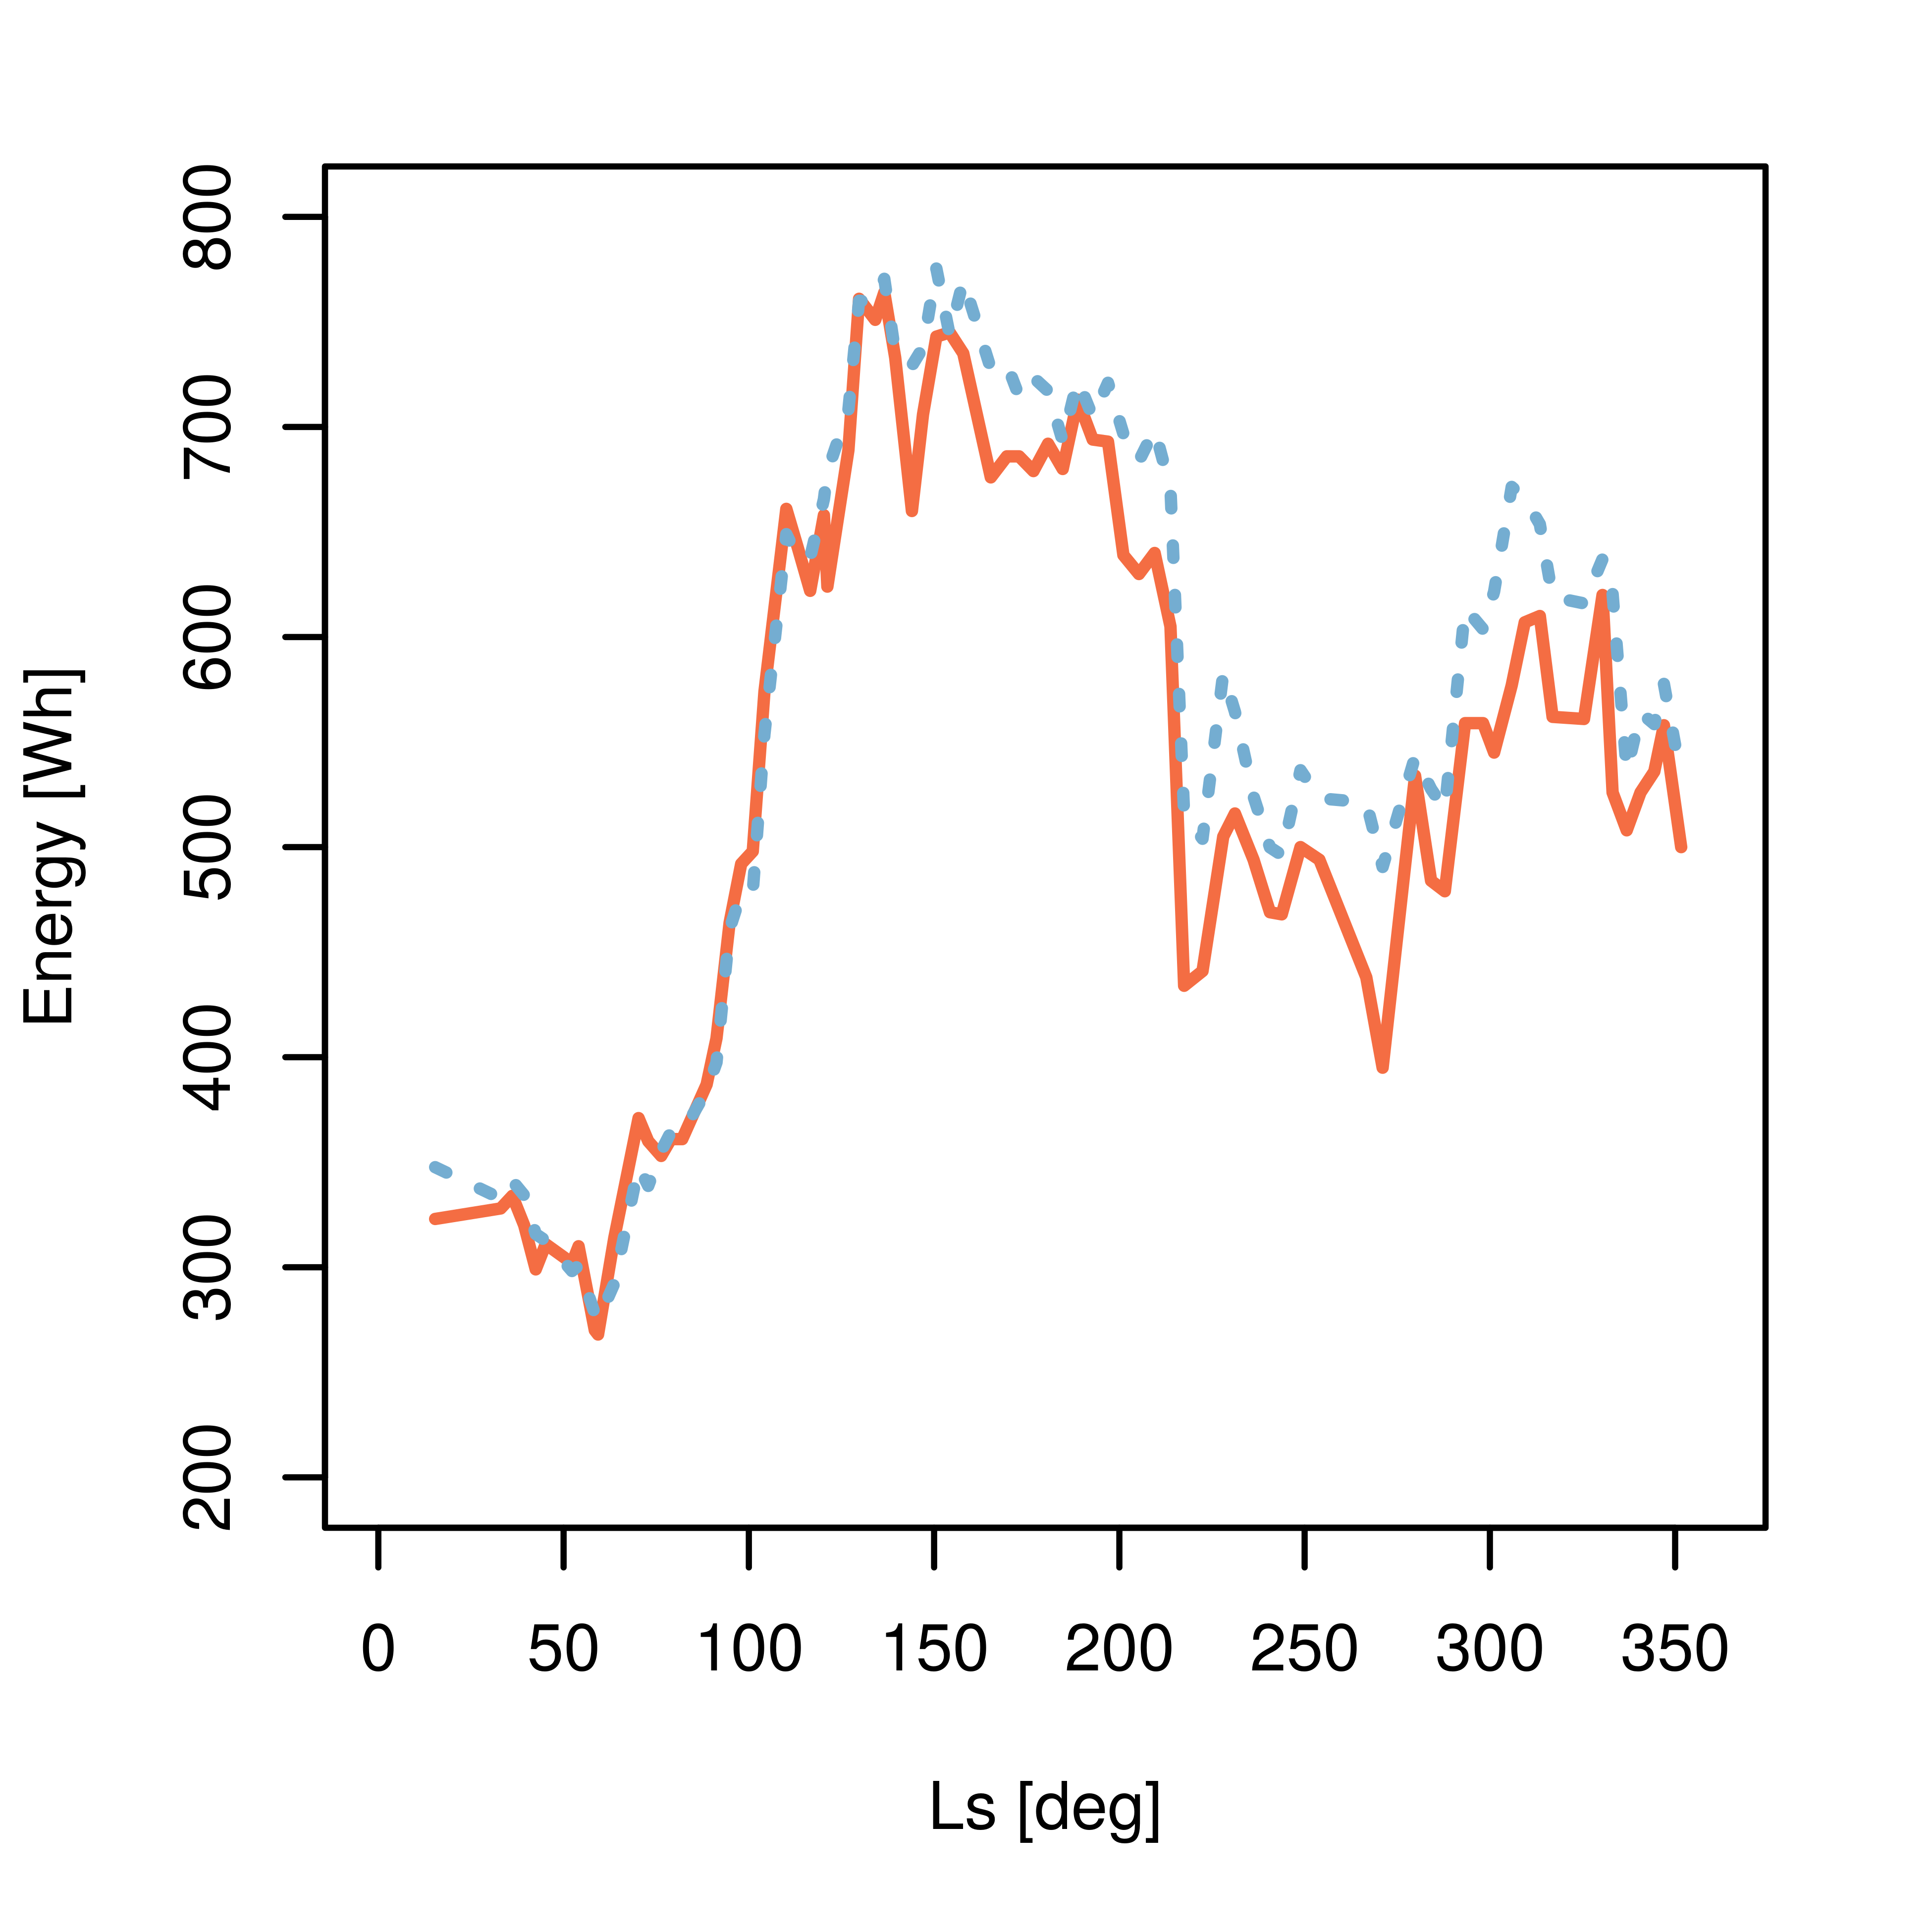
\includegraphics[height=\graphicsHeight]{sections/power-and-energy-predictions/plots/predicted-vs-measured-energy-my32.png}
  		\subcaption{MY32}
  		\label{fig:plot:sub:mer-energy-production-predicted-vs-reported-my32}
  	\end{subfigure}\hfill
	   \begin{subfigure}[t]{\subfigureWidth}
      \centering
  		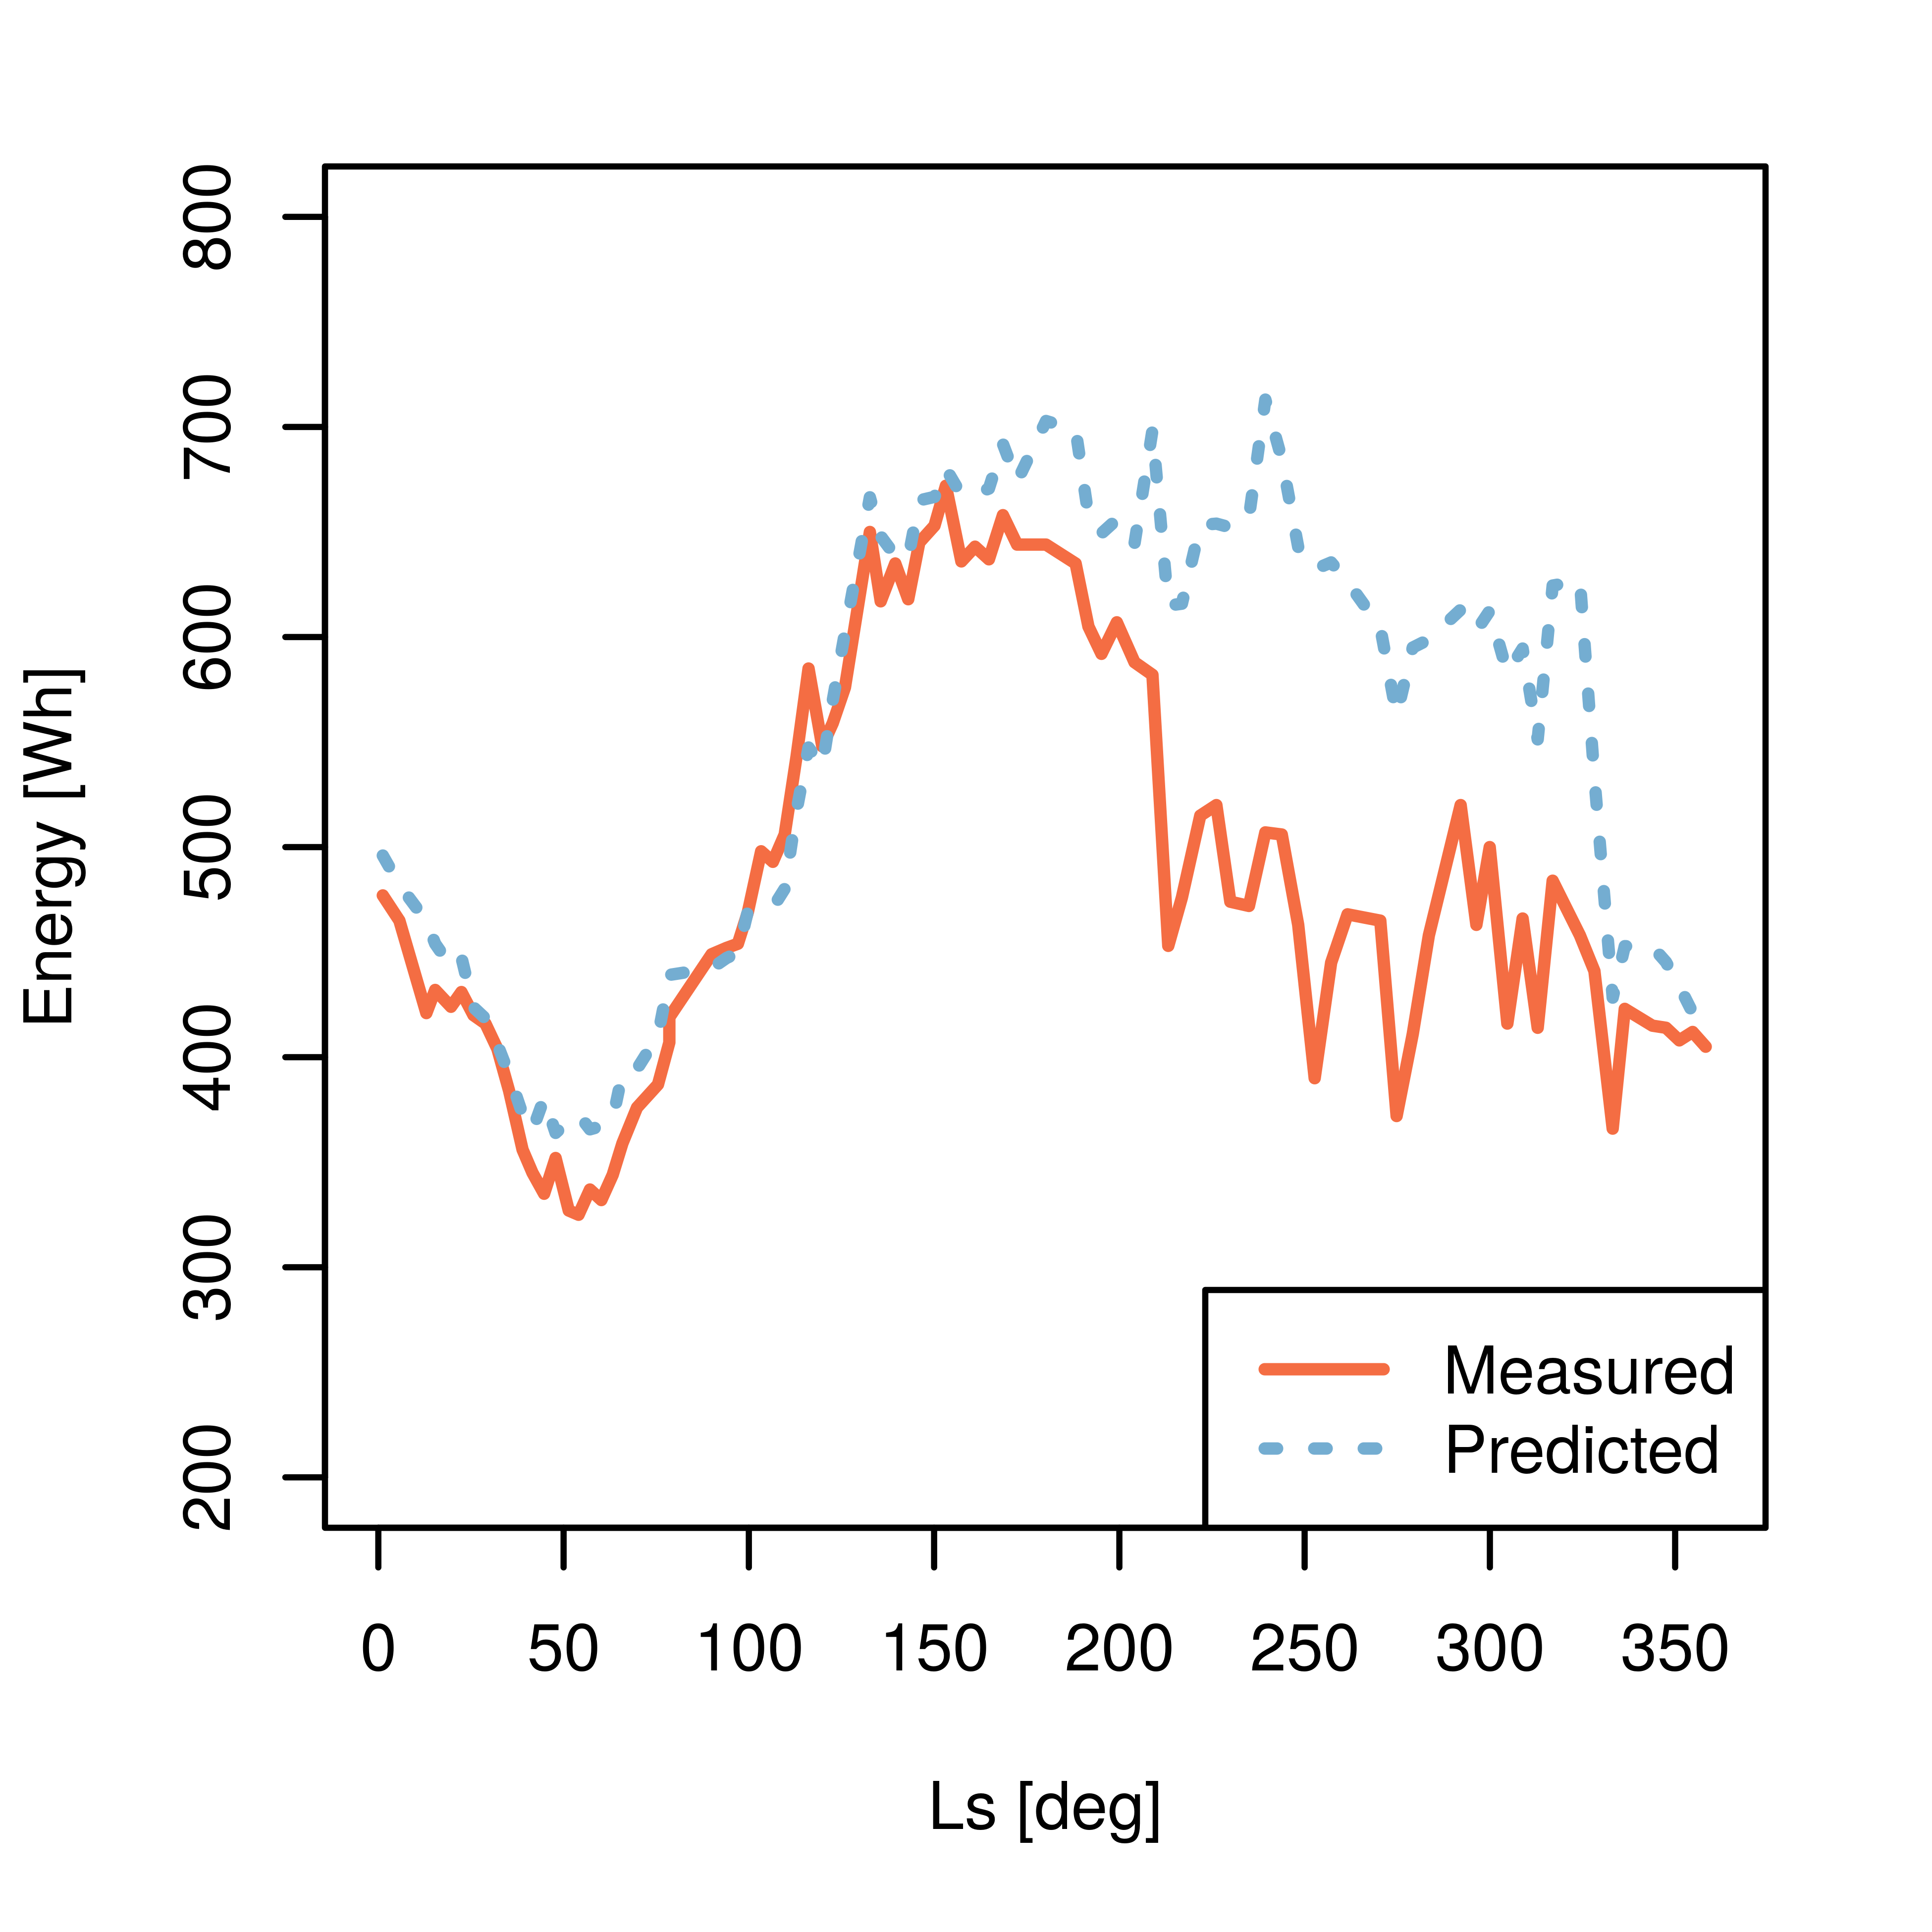
\includegraphics[height=\graphicsHeight]{sections/power-and-energy-predictions/plots/predicted-vs-measured-energy-my33.png}
  		\subcaption{MY33}
  		\label{fig:plot:sub:mer-energy-production-predicted-vs-reported-my33}
	   \end{subfigure}\hfill
    \caption[MER Opportunity PV energy production: predicted vs reported]
            {MER Opportunity PV energy production: predicted vs reported. Not shown are data for MY28 and MY34 which have also been scraped from the rover's status update logs.}
	\label{fig:plot:mer-energy-production-predicted-vs-reported}
\vspace{-2ex}
\end{figure}

\clearpage

A clear outlier is observed during the second half of MY33 in which predicted daily energy productions are much higher than what was reported. This is due to the rover's inclined descent through ``Bitterroot Valley'' during an intensive investigation into a gully at Endeavour Crater's western rim. Energy production predictions with horizontal surface Equation \ref{eq:SA_energy} not suited due to the inclination and orientation of such a descent. Applying Equation \ref{eq:SA_slope_energy} for $E_{\beta}$ would be more applicable. As such, data from MY33 is not considered in the validation exercise for horizontal surfaces.

\todo[inline]{TODO: Include reference to rover update for Bitterroot Valley descent.}
% Source: https://mars.nasa.gov/mer/mission/rover-status/opportunity/recent/all/?y=2016
% Source: https://www.nasa.gov/feature/jpl/rover-takes-on-steepest-slope-ever-tried-on-mars

Not included in Figure \ref{fig:plot:mer-energy-production-predicted-vs-reported} is data for MY34 during which the rover spent most of the year driving down ``Perseverance Valley'' on the west rim of Endeavour Crater. As was the case for MY33, applying Equation \ref{eq:SA_energy} for the MY34 would not be appropriate considering the rover's inclination during descents and is not considered in the validation exercise for horizontal surfaces.

% Source:https://mars.nasa.gov/mer/mission/rover-status/opportunity/recent/all/?y=2017
% Opportunity Remains at Current Location Due to Solar Conjunction
% sols 4787 to 4792, July 12, 2017 - July 17, 2017
% Opportunity entered Perseverance Valley on the west rim of Endeavour crater. The rover is positioned within the valley where she will spend the solar conjunction period.

Divergences from the predicted energy production are presented in Figure \ref{fig:plot:mer-energy-prediction-divergences} from which a -33\%/+7\% error margin range is observed. Negative values indicate predicted daily energy production greater than what was measured and the inverse is indicated by positive values.

\begin{figure}[h]
  \centering
  \hypersetup{linkcolor=captionTextColor}
  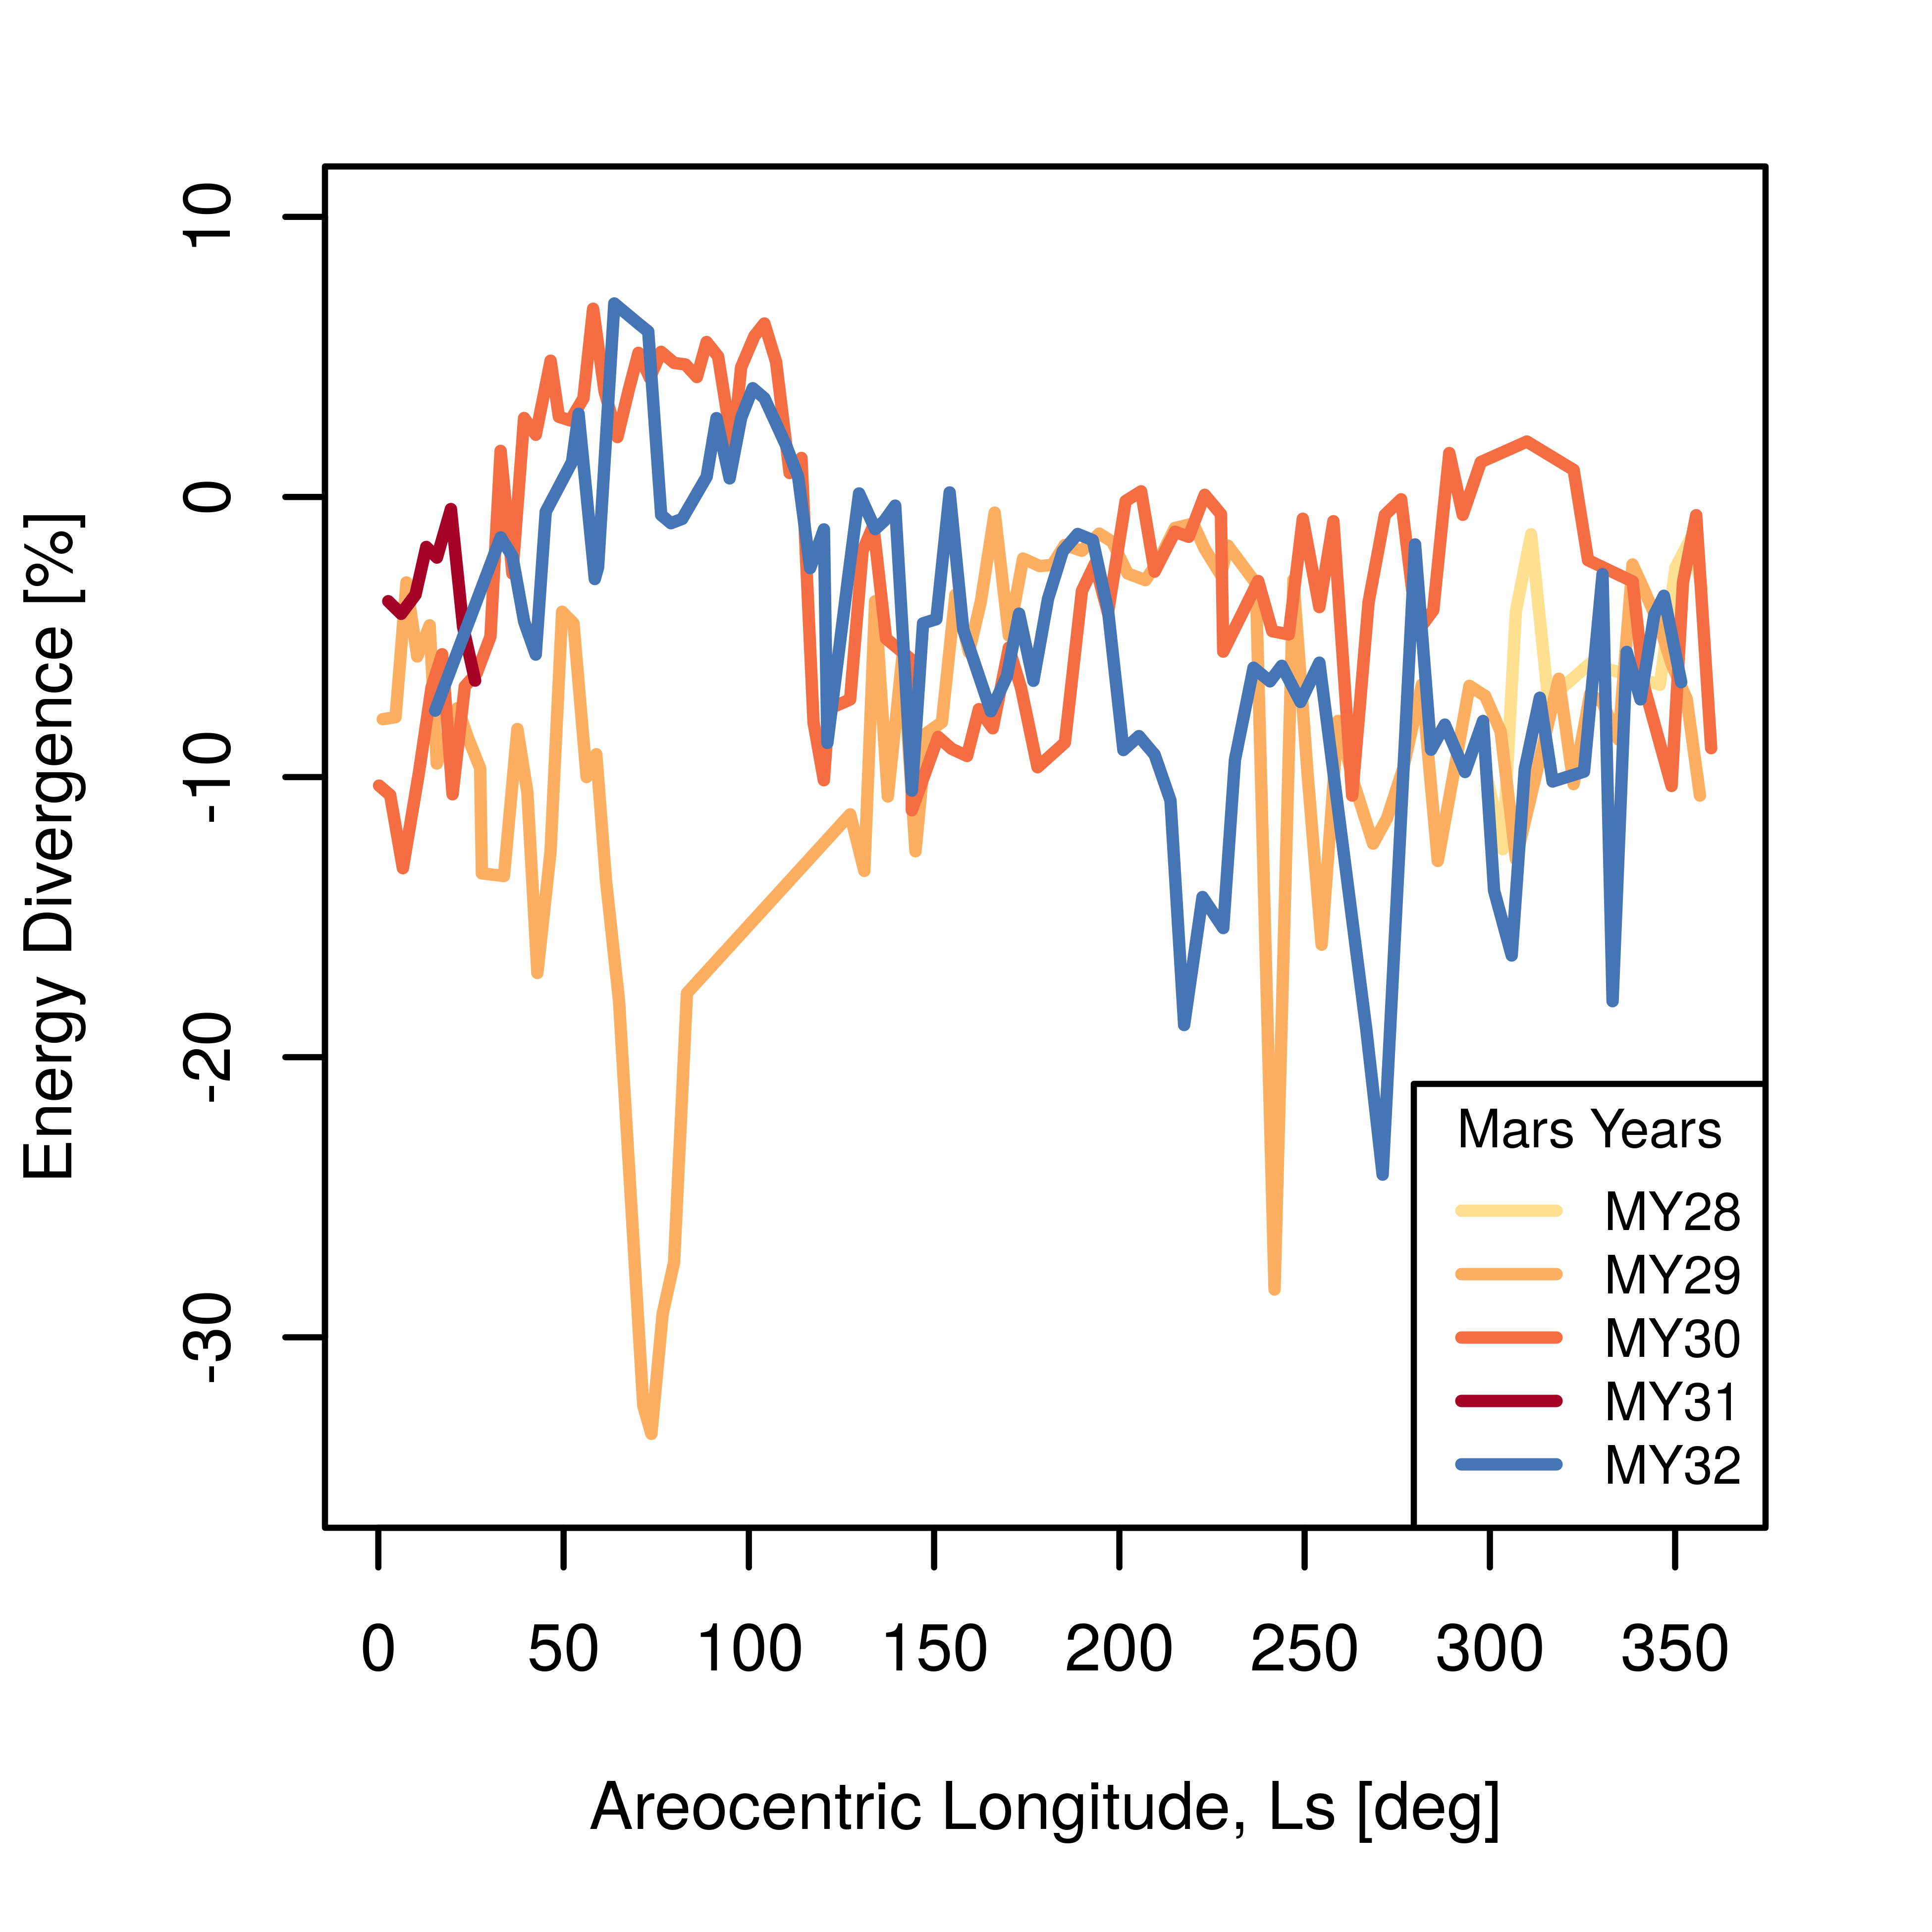
\includegraphics[width=0.8\linewidth]{sections/power-and-energy-predictions/plots/energy-prediction-divergences-from-my28-to-my32.png}\\
  \caption[Divergences from predicted MER Opportunity PV energy production]
          {Divergences from predicted MER Opportunity PV energy production.}
  \label{fig:plot:mer-energy-prediction-divergences}
\end{figure}

\clearpage

Figure \ref{fig:plot:binned-error-margins} bins the distribution of divergences across the -33\%/+7\% error margin range into 5\% increments. 65.5\% of the divergences occur within a -10\%/0\% error margin and 90.7\%  within -15\%/+5\%.

\begin{figure}[h]
  \centering
  \hypersetup{linkcolor=captionTextColor}
  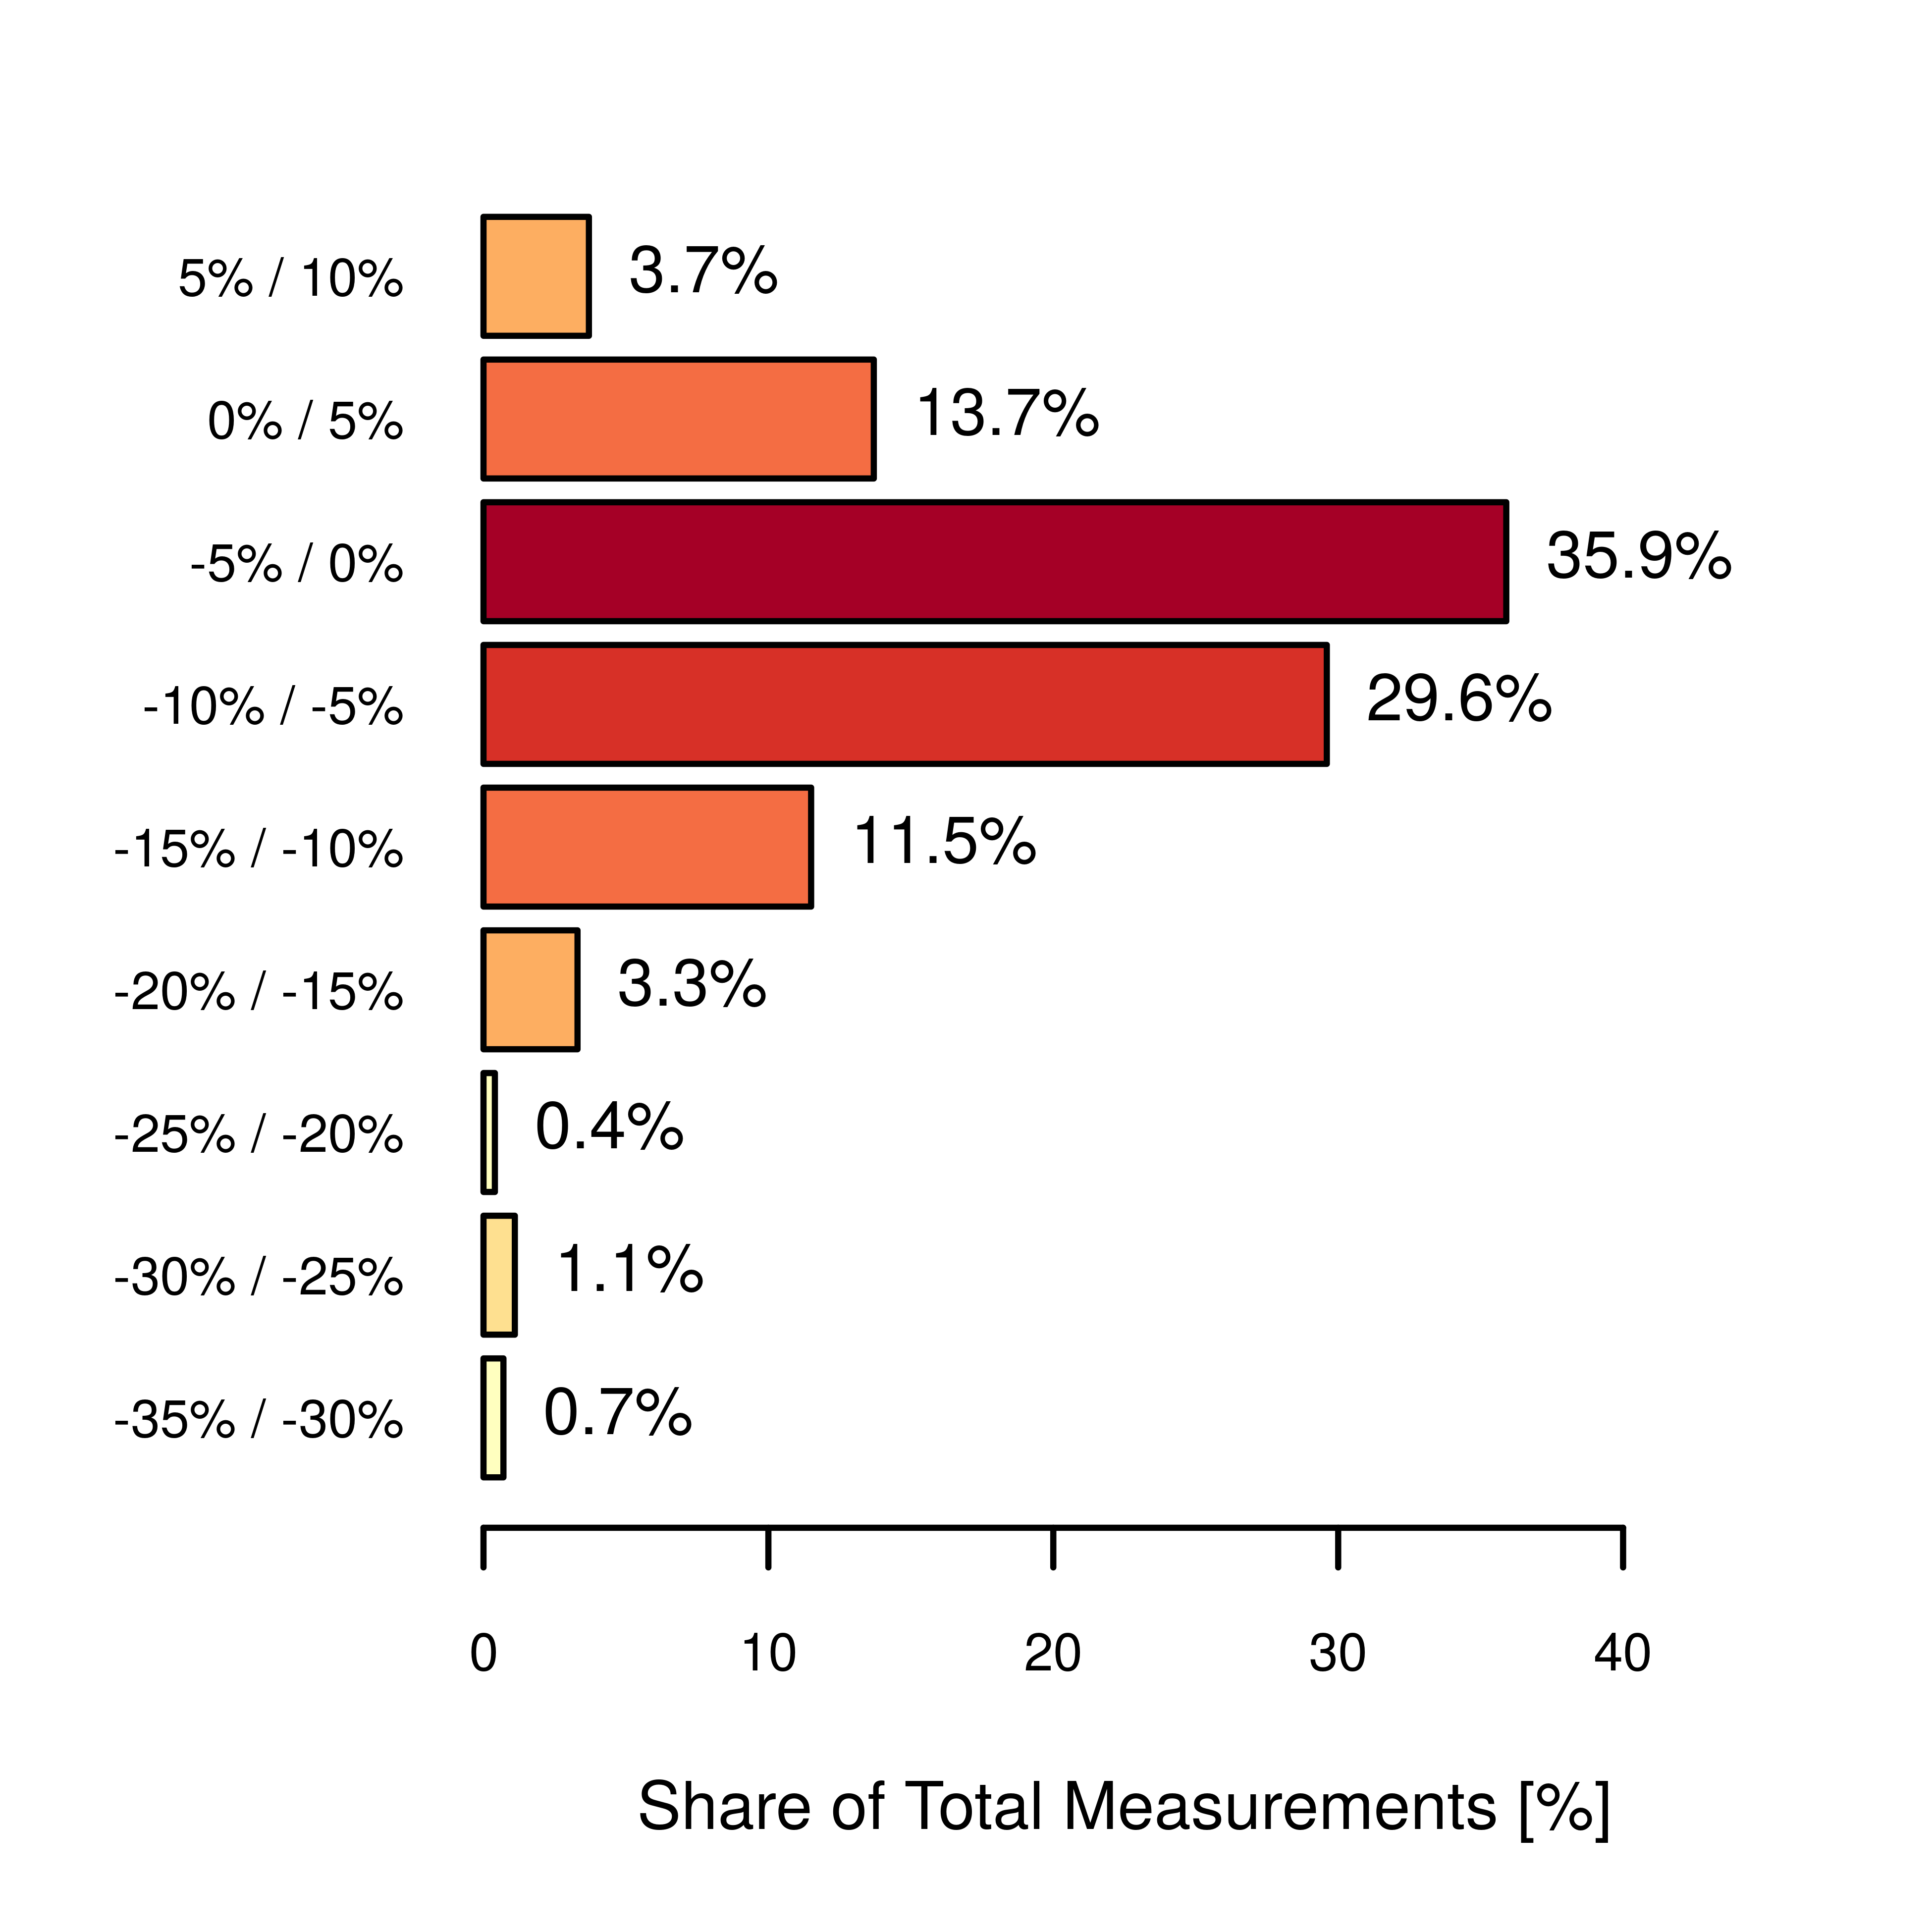
\includegraphics[width=0.8\linewidth]{sections/power-and-energy-predictions/plots/binned-error-margins.png}\\
  \caption[Binned error margins]
          {Binned error margins.}
  \label{fig:plot:binned-error-margins}
\end{figure}

The wide error margin range is thus a result of isolated local maxima outliers, notably at Sol 2204 (-33\%), 2218 (-27\%), 2519 (-28\%), and 3901 (-24\%). Table \ref{tab:divergences-less-than-m20pc} lists all divergences that are beyond -20\%.

\begin{table}[h]
    \centering
    \caption{Divergences from predicted MER Opportunity PV energy production that are beyond -20\%.}
    \label{tab:divergences-less-than-m20pc}
    \begin{tabular}{|l|c|c|c|c|c|c|c|}
    \hline
    \multicolumn{1}{|c|}{\multirow{2}{*}{\textbf{Date}}} & \multirow{2}{*}{\textbf{MY}} & \multirow{2}{*}{\textbf{Ls}} & \multirow{2}{*}{\textbf{Sol}} & \multicolumn{4}{c|}{\textbf{Energy [Wh]}} \\ \cline{5-8}
    \multicolumn{1}{|c|}{} &  &  &  & \textbf{Predicted} & \textbf{Measured} & \textbf{Diff.} & \textbf{Diff. [\%]} \\ \hline
    1-APR-2010 & 29 & 72 & 2199 & 315 & 238 & 77 & -32 \\
    6-APR-2010 & 29 & 74 & 2204 & 314 & 235 & 79 & -33 \\
    13-APR-2010 & 29 & 77 & 2211 & 293 & 227 & 66 & -29 \\
    20-APR-2010 & 29 & 80 & 2218 & 314 & 247 & 67 & -27 \\ \hline
    23-FEB-2011 & 29 & 242 & 2519 & 539 & 420 & 119 & -28 \\ \hline
    13-JAN-2015 & 32 & 271 & 3901 & 491 & 395 & 96 & -24 \\ \hline
    \end{tabular}
\end{table}


With the exception of Sol 2199 and 2218, possible explanations for large divergences beyond -20\% were obtained from MER Opportunity's status logs [?]:
\begin{enumerate}[(a)]
  \item Sol 2199: No turns or inclinations reported.
  \item Sol 2204: Turn - short sharp arc turn.
  \item Sol 2211: Inclination - crossed a series of ripples.
  \item Sol 2218: No turns or inclinations reported.
  \item Sol 2519: Turn - sharp repositioning turn.
  \item Sol 3901: Inclination - descended from the summit of 'Cape Tribulation'.
\end{enumerate}

\todo[inline]{TODO: Source MER Opportunity status log.}
%Sources. For terrestrial year 2010: https://mars.nasa.gov/mer/mission/rover-status/opportunity/2010/

The use of fixed daily values for the certain irradiance calculation variables also contributes to the observed divergences:
\begin{enumerate}[(a)]
  \item A fixed $\tau$ factor does not reflect the continuous changes in atmopheric optical depth.
  \item A fixed solar array dust factor does not reflect the irregularity of dust deposition over the entirety of the solar cell coverage area.
  \item A fixed shadowing performance loss coefficient does not reflect the diurnal changes in overshadowed area. Overshadowing changes throughout the day due to the position of the sun with respect to the location of the rover's petruding instruments, notably the Pancam Mast Assembly (PMA) as well as the low-gain and high-gain antennas.
\end{enumerate}

Attempts to narrow down the error margin range by adjusting the reported dust factor as well as shadowing and other losses are described in Appendix \ref{sec:Appendix:NarrowedEnergyPredictionErrorMarginRange}. However, these attempts resulted in overly conservative energy predictions and will not be applied.

By setting aside outliers causing divergences greater than 5\% and lesser than -15\% that were obtained with only 9.2\% of the dataset, the predicted energy production obtained with Equation \ref{eq:SA_energy} become acceptable for preliminary mission scenario analysis on a horizontal surfaces.

\clearpage
\subsection{Inclined Surface}
\label{sec:PowerAndEnergyPredictions:Validation:InclinedSurface}
\todo[inline]{TODO: Here we repeat the same exercise as in the previous section and compare if the obtained reduced error margins are similar. However, this is trickier because we don't have hundreds of data points since we lack slope angle data. Validation will have to be done at a micro level sich as when Opportunity's tilt hit 32 degrees on March 10, 2016, while making its closest approach to an intended target near the crest of 'Knudsen Ridge.'}

%Particularly while it was exploring steep outcrops within 'Marathon Valley' when the rover was inclined on the slopes of 'Knudsen Ridge' at Sol 4303 (March 1, 2016).
%The rover's tilt hit 32 degrees on March 10 while Opportunity was making its closest approach to an intended target near the crest of "Knudsen Ridge."
